\PassOptionsToPackage{no-math,cm-default}{fontspec}
\documentclass[twoside,nofonts,internet,shmeiwseis]{thewria}
\usepackage{amsmath}
\usepackage{xgreek}
\let\hbar\relax
\defaultfontfeatures{Mapping=tex-text,Scale=MatchLowercase}
\setmainfont[Mapping=tex-text,Numbers=Lining,Scale=1.0,BoldFont={Minion Pro Bold}]{Minion Pro}
\newfontfamily\scfont{GFS Artemisia}
\font\icon = "Webdings"
\usepackage[amsbb]{mtpro2}
\usepackage{tikz,pgfplots}
\tkzSetUpPoint[size=7,fill=white]
\xroma{red!70!black}
\setlist[itemize]{itemsep=0mm}
\newlist{rlist}{enumerate}{3}
\setlist[rlist]{itemsep=0mm,label=\roman*.}
\newlist{brlist}{enumerate}{3}
\setlist[brlist]{itemsep=0mm,label=\bf\roman*.}
\newlist{tropos}{enumerate}{3}
\setlist[tropos]{label=\bf\textit{\arabic*\textsuperscript{oς}\;Τρόπος :},leftmargin=0cm,itemindent=2.3cm,ref=\bf{\arabic*\textsuperscript{oς}\;Τρόπος}}
\newcommand{\tss}[1]{\textsuperscript{#1}}
\newcommand{\tssL}[1]{\MakeLowercase{\textsuperscript{#1}}}
\usepackage{hhline}
\usepackage{multicol,multirow}
\usepackage{wrap-rl,mathimatika,tkz-tab}
\usepackage{tikzpagenodes}
\usetkzobj{all}
\usepackage{tikz,tkz-euclide}
\usetikzlibrary{calc}
\usepackage{eso-pic}
\usepackage{comment}
\usepackage{venndiagram}
\usepackage{longtable,gensymb}
%------ Tikz - Item ----------------
%\begin{tikzpicture}[level/.style={sibling distance=50mm/#1},baseline]
%-----------------------------------
\usepackage{array}


%------ ΕΝΑΡΞΗ ΚΕΙΜΕΝΟΥ ----------
\begin{document}
\pagenumbering{gobble}% Remove page numbers (and reset to 1)
\clearpage
\titlos{Α΄ ΛΥΚΕΙΟΥ}{Αλγεβρα}{Ορισμοί και θεωρήματα}
\vspace{1cm}
\begin{center}
\begin{tikzpicture}
\begin{axis}[opacity=.5,aks_on,belh ar,xlabel={\footnotesize$x$},ylabel={\footnotesize$y$}
,xmin=-3,xmax=3.2,ymin=-3,ymax=3.2,x=1cm,y=1cm]
\addplot[opacity=.5,domain=-2:2,grafikh parastash]{x^2-1.4};
\addplot[opacity=.5,domain=-2:2,grafikh parastash]{x^2-2.2};
\end{axis}
\node at (1,2) {$x^2-Sx+p=0$};
\node at (5.5,4) {$P(A\cup B)=P(A)+P(B)-P(A\cap B)$};
\node at (-0.5,1) {$x_{1,2}=\dfrac{-\beta\pm\sqrt{\varDelta}}{2a}$};
\node at (5.5,1) {$|x|=\ccases{x & x\geq0\\-x & x<0}$};
\node at (0.5,5) {$S_\nu=\dfrac{\nu}{2}\left[2a_1+(\nu-1)\cdot\omega\right]$};
\node at (0,3.5) {$\sqrt[\nu]{a^\mu}=a^{\frac{\mu}{\nu}}$};
\node at (5.5,5.5) {$a_{\nu}=a_1\cdot\lambda^{\nu-1}$};
\node at (3.5,2.5) {$ \mathbb{Q}=\left\lbrace \left. \frac{a}{\beta}\right|a,\beta\in\mathbb{Z},\beta\neq0\;\right\rbrace  $};
\end{tikzpicture}\mbox{}\\
\vspace{3cm}
\begin{minipage}{7cm}
\begin{center}
ΑΝΑΛΥΤΙΚΟ ΤΥΠΟΛΟΓΙΟ ΓΙΑ ΤΗ ΘΕΩΡΙΑ ΤΗΣ ΑΛΓΕΒΡΑΣ Α΄ ΛΥΚΕΙΟΥ
\end{center}
\end{minipage}
\end{center}
\vspace*{\fill{\begin{center}
\end{center}}}
\newpage\phantom{}
\vspace{7cm}
\begin{center}
\begin{flushright}
\begin{minipage}{7cm}
\textit{Αεί ο Θεός ο Μέγας γεωμετρεί,
το κύκλου μήκος ίνα ορίση διαμέτρω,
παρήγαγεν αριθμόν απέραντον,
καί όν, φεύ,
ουδέποτε όλον θνητοί θα εύρωσι.}
\[ \pi=3{,}1415926535897932384626 \]
Το πλήθος των γραμμάτων κάθε λέξης στην παραπάνω πρόταση φτιάχνουν διαδοχικά τα 23 πρώτα ψηφία του αριθμού $ \pi $.
\end{minipage}
\end{flushright}
\end{center}
\newpage\phantom{}
\pagenumbering{arabic}
\section{Σύνολα - Πιθανότητες}
\begin{enumerate}
\item \textbf{Σύνολο:} Συλλογή όμοιων αντικειμένων.
\begin{itemize}[itemsep=0mm]
\item Τα αντικείμενα λέγονται \textbf{στοιχεία}.
\item Τα σύνολα τα συμβολίζουμε με ένα κεφαλαίο γράμμα.
\item Το $ x $ \textbf{ανήκει} στο σύνολο $ A $: $ x\in A $.
\item \textbf{Κενό:} Το σύνολο χωρίς στοιχεία : $ \varnothing $.
\item \textbf{Βασικό:} Το σύνολο που περιέχει όλα τα στοιχεία: $ \varOmega $.
\end{itemize}
\textbf{ΒΑΣΙΚΑ ΣΥΝΟΛΑ ΑΡΙΘΜΩΝ}
\begin{multicols}{2}
\begin{brlist}[leftmargin=4mm]
\item \textbf{Φυσικοί Αριθμοί} : $ \mathbb{N}=\{0,1,2,3,\ldots\} $.
\item \textbf{Ακέραιοι Αριθμοί} : $ \mathbb{Z}=\{\ldots,-2,-1,0,1,2,\ldots\} $.
\item \textbf{Ρητοί Αριθμοί} : $ \mathbb{Q}=\left\lbrace \left. \frac{a}{\beta}\right|a,\beta\in\mathbb{Z},\beta\neq0\;\right\rbrace  $.
\item \textbf{Άρρητοι Αριθμοί} : Κάθε αριθμός που δεν είναι ρητός.
\item \textbf{Πραγματικοί Αριθμοί} : $\mathbb{R}=\{ \textrm{όλοι οι αριθμοί} \} $.
\end{brlist}
\end{multicols}
\item \textbf{Ίσα σύνολα:} $ A=B $ αν έχουν τα ίδια στοιχεία. 
\item \textbf{Υποσύνολο:} $ A\subseteq B $.
\item \textbf{Πράξεις μεταξύ συνόλων}
\begin{brlist}
\item \textbf{Ένωση:} $ A\cup B=\left\lbrace x\in\varOmega\left| x\in A \textrm{ ή } x\in B\right.\right\rbrace $
\item \textbf{Τομή:} $ A\cap B=\left\lbrace x\in\varOmega\left| x\in A \textrm{ και } x\in B\right.\right\rbrace $
\item \textbf{Συμπλήρωμα:} $ A'=\left\lbrace x\in\varOmega\left| x\notin A\right.\right\rbrace $
\item \textbf{Διαφορά:} $ A-B=\left\lbrace x\in\varOmega\left| x\in A\textrm{ και }x\notin B\right. \right\rbrace $
\end{brlist}
\end{enumerate}
\section{Πραγματικοί Αριθμοί}
\begin{enumerate}
\item \textbf{Δύναμη πραγματικού αριθμού:} $ a\cdot a\cdot\ldots a=a^\nu $. Ο $ a $ λέγεται \textbf{βάση} και ο $ \nu $ \textbf{εκθέτης}.
\item \textbf{Ταυτότητα:} Μια ισότητα που περιέχει μεταβλητές και επαληθεύεται για κάθε τιμή των μεταβλητών.
\begin{multicols}{2}
\begin{enumerate}[itemsep=0mm,label=\bf\arabic*.]
\item \parbox[t]{7cm}{\textbf{Άθροισμα στο τετράγωνο}\\$ (a+\beta)^2=a^2+2a\beta+\beta^2 $}
\item \parbox[t]{7cm}{\textbf{Διαφορά στο τετράγωνο}\\$ (a-\beta)^2=a^2-2a\beta+\beta^2 $}
\item \parbox[t]{7cm}{\textbf{Άθροισμα στον κύβο}\\$ (a+\beta)^3=a^3+3a^2\beta+3a\beta^2+\beta^3 $}
\item \parbox[t]{7cm}{\textbf{Διαφορά στον κύβο}\\$ (a-\beta)^3=a^3-3a^2\beta+3a\beta^2-\beta^3 $}
\item \parbox[t]{7cm}{\textbf{Γινόμενο αθροίσματος επί διαφορά}\\$ (a+\beta)(a-\beta)=a^2-\beta^2 $}
\item \parbox[t]{7cm}{\textbf{Άθροισμα κύβων}\\$ (a+\beta)\left(a^2-a\beta+\beta^2 \right)=a^3+\beta^3 $}
\item \parbox[t]{7cm}{\textbf{Διαφορά κύβων}\\$ (a-\beta)\left(a^2+a\beta+\beta^2 \right)=a^3-\beta^3 $}
\end{enumerate}
\end{multicols}
\item \textbf{Παραγοντοποίηση αλγεβρικών παραστάσεων}
Η διαδικασία με την οποία μια αλγεβρική παράσταση μετατρέπεται από άθροισμα σε γινόμενο.
\item \textbf{Διάστημα - κέντρο - ακτίνα διαστήματος}
\begin{itemize}[itemsep=0mm]
\item Ο αριθμός $ x_0=\frac{a+\beta}{2} $ ονομάζεται \textbf{κέντρο}, ο αριθμός $ \mu=\beta-a $ ονομάζεται \textbf{μήκος} και ο αριθμός $ \rho=\frac{\beta-a}{2} $ ονομάζεται \textbf{ακτίνα} του διαστήματος.
\end{itemize}
\begin{center}
\begin{longtable}{cc>{\centering\arraybackslash}m{4cm}c}
\hline \rule[-2ex]{0pt}{5.5ex} \textbf{Διάστημα} & \textbf{Ανισότητα} & \textbf{Σχήμα} & \textbf{Περιγραφή} \\ 
\hhline{====} \rule[-2ex]{0pt}{5.5ex} $ [a,\beta] $ & $ a\leq x\leq\beta $ & \begin{tikzpicture}
\tkzDefPoint(0,.57){A}
\diasthma{a}{ \beta }{.7}{2.3}{.3}{\xrwma}
\axonas{0}{3}
\akro{k}{.7}
\akro{k}{2.3}
\end{tikzpicture} & Κλειστό $ a,\beta $ \\ 
$ (a,\beta) $ & $ a< x<\beta $ & \begin{tikzpicture}
\tkzDefPoint(0,.57){A}
\diasthma{a}{ \beta }{.7}{2.3}{.3}{\xrwma}
\axonas{0}{3}
\akro{a}{.7}
\akro{a}{2.3}
\end{tikzpicture} & Ανοιχτό $ a,\beta $\\
$ [a,\beta) $ & $ a\leq x<\beta $ & \begin{tikzpicture}
\tkzDefPoint(0,.57){A}
\diasthma{a}{ \beta }{.7}{2.3}{.3}{\xrwma}
\axonas{0}{3}
\akro{k}{.7}
\akro{a}{2.3}
\end{tikzpicture} & Κλειστό $a$ ανοιχτό $\beta$\\
$ (a,\beta] $ & $ a< x\leq\beta $ & \begin{tikzpicture}
\tkzDefPoint(0,.57){A}
\diasthma{a}{ \beta }{.7}{2.3}{.3}{\xrwma}
\axonas{0}{3}
\akro{a}{.7}
\akro{k}{2.3}
\end{tikzpicture} & Ανοιχτό $a$ κλειστό $\beta$ \\
$ [a,+\infty) $ & $ x\geq a $ & \begin{tikzpicture}
\tkzDefPoint(0,.57){A}
\Xapeiro{a}{.7}{3}{.3}{\xrwma}
\axonas{0}{3}
\akro{k}{.7}
\end{tikzpicture} & Κλειστό $a$ συν άπειρο \\
$ (a,+\infty) $ & $ x>a $ & \begin{tikzpicture}
\tkzDefPoint(0,.57){A}
\Xapeiro{a}{.7}{3}{.3}{\xrwma}
\axonas{0}{3}
\akro{a}{.7}
\end{tikzpicture} & Ανοιχτό $a$ συν άπειρο \\
$ (-\infty,a] $ & $ x\leq a $ & \begin{tikzpicture}
\tkzDefPoint(0,.57){A}
\apeiroX{a}{2.3}{0}{.35}{\xrwma}
\axonas{0}{3}
\akro{k}{2.3}
\end{tikzpicture} & Μείον άπειρο $a$ κλειστό \\
$ (-\infty,a) $ & $ x<a $ & \begin{tikzpicture}
\tkzDefPoint(0,.57){A}
\apeiroX{a}{2.3}{0}{.35}{\xrwma}
\axonas{0}{3}
\akro{a}{2.3}
\end{tikzpicture} & Μείον άπειρο $a$ ανοιχτό \\
\hline 
\end{longtable}
\end{center}
\vspace{-5mm}
\item \item \textbf{απολυτη τιμη πραγματικου αριθμου} απόστασή του απο το $ 0 $.
\begin{center}
\begin{tabular}{c >{\centering\arraybackslash}m{6cm}}
$ |a|=\begin{cases}
\begin{aligned}
a & \;,\;a\geq0\\
-a & \;,\;a<0
\end{aligned}
\end{cases} $  & 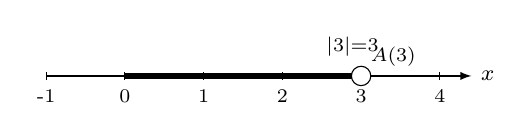
\begin{tikzpicture}
\draw[-latex] (-1,0) -- coordinate (x axis mid) (4.4,0) node[right,fill=white] {{\footnotesize $ x $}};
\foreach \x in {-1,0,...,4}
\draw (\x,.5mm) -- (\x,-.5mm) node[anchor=north,fill=white] {{\scriptsize \x}};
\draw[line width=.7mm] (0,0) -- (3,0);
\tkzText(1.5,.34){$ \overcbrace{\rule{28mm}{0mm}}^{{\scriptsize |3|=3}} $}
\tkzDefPoint(3,0){A}
\tkzDrawPoint[size=7,fill=white](A)
\tkzLabelPoint[above right](A){{\scriptsize $A(3)$}}
\end{tikzpicture}
\end{tabular} 
\end{center}
Η απόσταση δύο αριθμών μεταξύ τους ορίζεται ως η απόλυτη τιμή της διαφοράς τους.
\[ |a-\beta|=d(a,\beta) \]
\Orismos{Τετραγωνική Ρίζα:} 
$ \sqrt{x}=a\;\;,\;\;\textrm{ όπου }x\geq0\textrm{ και }a\geq0 $
\begin{itemize}[itemsep=0mm]
\item Ο αριθμός $ x $ ονομάζεται \textbf{υπόριζο}.
\item Δεν ορίζεται ρίζα αρνητικού αριθμού.
\end{itemize}
\item \textbf{ριζα \MakeLowercase{ν}-ταξησ πραγματικου αριθμου} $ \sqrt[\nu]{x}=a\;\;,\;\;\textrm{ όπου }x\geq0\textrm{ και }a\geq0 $.
\item \textbf{Δυναμη με ρητό εκθετη} $ a^{\frac{\mu}{\nu}}=\!\sqrt[\nu]{a^\mu}\ ,\ \textrm{ όπου } a>0  $
\thewrhmata
\Thewrhma{Ιδιότητεσ των Πράξεων}
\begin{center}
\begin{tabular}{ccc}
\hline \rule[-2ex]{0pt}{5.5ex} \textbf{Ιδιότητα} & \textbf{Πρόσθεση} & \textbf{Πολλαπλασιασμός} \\ 
\hhline{===} \rule[-2ex]{0pt}{5.5ex} \textbf{Αντιμεταθετική} & $ a+\beta=\beta+a $ & $ a\cdot\beta=\beta\cdot a $ \\
\rule[-2ex]{0pt}{5ex} \textbf{Προσεταιριστική} & $ a+\left( \beta+\gamma\right) =\left( a+\beta\right) +\gamma $ & $ a\cdot\left( \beta\cdot\gamma\right) =\left( a\cdot\beta\right)\cdot\gamma $\\
\rule[-2ex]{0pt}{5ex} \textbf{Ουδέτερο στοιχείο} & $ a+0=a $ & $ a\cdot1= a $\\
\rule[-2ex]{0pt}{5ex} \textbf{Αντίθετοι / Αντίστροφοι} & $ a+(-a)=0 $ & $ a\cdot\frac{1}{a}= 1 $\\
\rule[-2ex]{0pt}{5ex} \textbf{Επιμεριστική} & \multicolumn{2}{c}{$ a\cdot\left( \beta\pm\gamma\right)=a\cdot\beta\pm a\cdot\gamma  $}\\
\hline
\end{tabular}
\end{center}
Ισχύουν επίσης :
\begin{itemize}[itemsep=0mm]
\item Για κάθε πραγματικό αριθμό $ a $ ισχύει $ a\cdot0=0 $
\item Δύο αριθμοί που έχουν άθροισμα 0 λέγονται \textbf{αντίθετοι}.
\item Το 0 λέγεται \textbf{ουδέτερο στοιχείο της πρόσθεσης}.
\item Δύο αριθμοί που έχουν γινόμενο 1 λέγονται \textbf{αντίστροφοι}.
\item Το 1 λέγεται \textbf{ουδέτερο στοιχείο του πολλαπλασιασμού}.
\item Το 0 δεν έχει αντίστροφο.
\end{itemize}
\Thewrhma{Ιδιότητεσ ισοτήτων}
\begin{rlist}
\item Τοποθετούμε τον ίδιο αριθμό και στα δύο μέλη της με πρόσθεση, αφαίρεση, πολλαπλασιασμό ή διαίρεση.
\[ a=\beta\Rightarrow
\begin{cases}
a+\gamma=\beta+\gamma\\a-\gamma=\beta-\gamma
\end{cases}\ \ \textrm{ και }\ \ \begin{aligned}
&a\cdot\gamma=\beta\cdot\gamma\\&\dfrac{a}{\gamma}=\dfrac{\beta}{\gamma}\;\;,\;\;\gamma\neq0
\end{aligned} \]
\item Εαν δύο πραγματικοί αριθμοί $ a,\beta\in\mathbb{R} $ είναι ίσοι τότε και οι ν-οστές δυνάμεις τους, $ \nu\in\mathbb{N} $, θα είναι ίσες. Το αντίστροφο δεν ισχύει πάντα.
\begin{gather*}
a=\beta\Rightarrow a^\nu=\beta^\nu
\end{gather*}
\item Εαν δύο θετικοί πραγματικοί αριθμοί $ a,\beta>0 $ είναι ίσοι τότε και οι ν-οστές ρίζες τους, $ \nu\in\mathbb{N} $, θα είναι με ίσες και αντίστροφα.
\begin{gather*}
a=\beta\Leftrightarrow\sqrt[\nu]{a}=\!\sqrt[\nu]{\beta}
\end{gather*}
\end{rlist}
\Thewrhma{Πράξεισ μεταξύ ισοτήτων}
\[ a=\beta\;\;\textrm{και}\;\;\gamma=\delta\Rightarrow
\ccases{
\textrm{\textbf{{1. Πρόσθεση κατά μέλη }}}& a+\gamma=\beta+\delta\\\textrm{\textbf{{2. Αφαίρεση κατά μέλη }}}& a-\gamma=\beta-\delta\\\textrm{\textbf{{3. Πολλαπλασιασμός κατά μέλη }}}& a\cdot\gamma=\beta\cdot\delta\\\textrm{\textbf{{4. Διαίρεση κατά μέλη }}}& \dfrac{a}{\gamma}=\dfrac{\beta}{\delta}\;\;,\;\;\gamma\cdot\delta\neq0} \]
\Thewrhma{Νόμοσ διαγραφησ προσθεσησ \& πολλαπλασιασμου}
\[ a+x=a+y\Rightarrow x=y\;\;\textrm{ και }\;\;a\cdot x=a\cdot y\Rightarrow x=y \]
\Thewrhma{μηδενικό γινόμενο}
\[ a\cdot\beta=0\Leftrightarrow a=0\textrm{ \textbf{ή} }\beta=0 \]
\Thewrhma{μη μηδενικο γινόμενο}
\[ a\cdot\beta\neq0\Leftrightarrow a\neq0\textrm{ \textbf{και} }\beta\neq0 \]
\Thewrhma{Ιδιότητεσ δυνάμεων}
\[ a^1=a\;\;,\;\;a^0=1\;,\;\textrm{όπου }a\neq0\;\;,\;\;a^{-\nu}=\dfrac{1}{a^\nu}\;,\;\textrm{όπου }a\neq0 \]
\begin{center}
\begin{longtable}{ccc}
\hline \rule[-2ex]{0pt}{5.5ex} & \textbf{Ιδιότητα} & \textbf{Συνθήκη} \\
\hhline{===}\rule[-2ex]{0pt}{5.5ex} \textbf{1} & Γινόμενο δυνάμεων με κοινή βάση & $ a^\nu\cdot a^\mu=a^{\nu+\mu} $ \\
\rule[-2ex]{0pt}{5.5ex} \textbf{2} & Πηλίκο δυνάμεων με κοινή βάση & $ a^\nu: a^\mu=a^{\nu-\mu} $\\
\rule[-2ex]{0pt}{5.5ex} \textbf{3} & Γινόμενο δυνάμεων με κοινό εκθέτη & $ \left(a\cdot\beta\right)^\nu=a^\nu\cdot\beta^\nu $ \\
\rule[-2ex]{0pt}{5.5ex} \textbf{4} & Πηλίκο δυνάμεων με κοινό εκθέτη & $ \left(\dfrac{a}{\beta}\right)^\nu=\dfrac{a^\nu}{\beta^\nu}\;\;,\;\;\beta\neq0 $ \\
\rule[-2ex]{0pt}{5.5ex} \textbf{5} & Δύναμη υψωμένη σε δύναμη & $ \left( a^\nu\right)^\mu=a^{\nu\cdot\mu} $ \\
\rule[-2ex]{0pt}{5.5ex} \textbf{6} & Κλάσμα με αρνητικό εκθέτη & $ \left( \dfrac{a}{\beta}\right)^{-\nu}=\left(\dfrac{\beta}{a}\right)^\nu\;\;,\;\;a,\beta\neq0 $ \vspace{2mm}\\
\hline
\end{longtable}
\end{center}
\vspace{-10mm}
\Thewrhma{Ιδιότητεσ διάταξησ}
\begin{enumerate}
\item Αν $ a>\beta $ και $ \beta>\gamma \Rightarrow a>\gamma $. (Μεταβατική ιδιότητα).
\item 
\begin{rlist}
\item Αν $ a>0 $ και $ \beta>0 $ τότε $ a+\beta>0 $.
\item Αν $ a<0 $ και $ \beta<0 $ τότε $ a+\beta<0 $.
\end{rlist}
\item Αν $ a,\beta\ \textrm{ομόσημοι}\ \Leftrightarrow a\cdot\beta>0\ \textrm{και}\ \frac{a}{\beta}>0 $.
\item Αν $ a,\beta\ \textrm{ετερόσημοι}\ \Leftrightarrow a\cdot\beta<0\ \textrm{και}\ \frac{a}{\beta}<0 $.
\item Αν $ a>\beta\Leftrightarrow a+\gamma>\beta+\gamma\ \textrm{και}\ a-\gamma>\beta-\gamma $.
\item 
\begin{rlist}
\item $ \textrm{Αν }\gamma>0\textrm{ τότε }a>\beta\Leftrightarrow a\cdot\gamma>\beta\cdot\gamma\textrm{ και }\dfrac{a}{\gamma}>\dfrac{\beta}{\gamma} $
\item $ \textrm{Αν }\gamma<0\textrm{ τότε }a>\beta\Leftrightarrow a\cdot\gamma<\beta\cdot\gamma\textrm{ και }\dfrac{a}{\gamma}<\dfrac{\beta}{\gamma} $
\end{rlist}
\item \begin{rlist}
\item $ \textrm{Αν }a,\beta\textrm{ ομόσημοι τότε } a>\beta\Leftrightarrow \dfrac{1}{a}<\dfrac{1}{\beta} $
\item $ \textrm{Αν }a,\beta\textrm{ ετερόσημοι τότε } a>\beta\Leftrightarrow \dfrac{1}{a}>\dfrac{1}{\beta} $
\end{rlist}
\end{enumerate}
Ανάλογα συμπεράσματα ισχύουν και για τις ανισότητες $ a<\beta,a\geq\beta $ και $ a\leq\beta $.\\\\
\Thewrhma{Πράξεισ κατά μέλη ανισοτήτων}
\[ a>\beta\;\;\textrm{και}\;\;\gamma>\delta\Rightarrow\begin{cases}
\textrm{\textbf{{1. Πρόσθεση κατά μέλη }}}& a+\gamma>\beta+\delta\\\textrm{\textbf{{2. Πολλαπλασιασμός κατά μέλη }}}& a\cdot\gamma>\beta\cdot\delta\;\;,\;\;\textrm{με }a,\beta,\gamma,\delta>0
\end{cases} \]
\textbf{Δεν} μπορούμε να αφαιρέσουμε ή να διαιρέσουμε ανισότητες κατά μέλη.\\\\
\Thewrhma{Δύναμη με άρτιο εκθέτη}
\[ a^2\geq0\ \ ,\ \ a^{2\kappa}\geq0\;\;,\;\;\kappa\in\mathbb{Z} \]
\Thewrhma{Άθροισμα δυνάμεων με άρτιο εκθέτη}
 \[ a^2+\beta^2\geq0 \]
\Thewrhma{ιδιοτητεσ απολυτων τιμων}
\begin{center}
\begin{longtable}{ccc}
\hline \rule[-2ex]{0pt}{5.5ex} & \textbf{Ιδιότητα} & \textbf{Συνθήκη} \\
\hhline{===}\rule[-2ex]{0pt}{5.5ex} \textbf{1} & Πρόσημο απόλυτης τιμής & $ |a|=|-a|\geq0 $ \\
\rule[-2ex]{0pt}{5.5ex} \textbf{2} & Απόλυτη τιμή μηδενός & $ |a|=0\Leftrightarrow a=0 $\\
\rule[-2ex]{0pt}{5.5ex} \textbf{3} & Όρια αριθμού & $ -|a|\leq a\leq|a| $ \\
\rule[-2ex]{0pt}{5.5ex} \textbf{4} & Απόλυτη τιμή γινομένου & $ |a\cdot\beta|=|a|\cdot|\beta| $ \\
\rule[-2ex]{0pt}{5.5ex} \textbf{5} & Απόλυτη τιμή πηλίκου & $ \left| \dfrac{a}{\beta}\right|=\dfrac{|a|}{|\beta|} $ \\
\rule[-2ex]{0pt}{5.5ex} \textbf{6} & Τετράγωνο απόλυτης τιμής & $ |a|^2=a^2 $ \\
\rule[-2ex]{0pt}{5.5ex} \textbf{7} & Τριγωνική ανισότητα & $ \left||a-\beta| \right|\leq|a\pm\beta|\leq|a|+|\beta|  $ \\
\hline
\end{longtable}
\end{center}
\Thewrhma{Ιδιότητεσ Ριζών}
\begin{center}
\begin{longtable}{ccc}
\hline \rule[-2ex]{0pt}{5.5ex} & \textbf{Ιδιότητα} & \textbf{Συνθήκη} \\
\hhline{===}\rule[-2ex]{0pt}{5.5ex} \textbf{1} & Τετράγωνο ρίζας & $ \left(\!\sqrt{x}\;\right)^2=x\;\;,\;\; x\geq0  $ \\
\rule[-2ex]{0pt}{5.5ex} \textbf{2} & Ν-οστή δύναμη ν-οστής ρίζας & $ \left(\!\sqrt[\nu]{x}\;\right)^\nu=x\;\;,\;\; x\geq0  $ \\
\rule[-2ex]{0pt}{5.5ex} \textbf{3} & Ρίζα τετραγώνου & $ \sqrt{x^2}=|x|\;\;,\;\; x\in\mathbb{R} $\\
\rule[-2ex]{0pt}{5.5ex} \textbf{4} & Ν-οστή ρίζα ν-οστής δύναμης & $ \sqrt[\nu]{x^\nu}=\begin{cases}
|x|&  x\in\mathbb{R}\textrm{ αν }\nu\textrm{ άρτιος}\\x&  x\geq0\textrm{ και } \nu\in\mathbb{N}\end{cases} $\\
\hhline{~~-} \multirow{3}{*}{\textbf{5}} & \multirow{3}{*}{Ρίζα γινομένου} & $ \sqrt{x\cdot y}=\!\sqrt{x}\cdot\!\sqrt{y}\;\;,\;\; x,y\geq0 $ \rule[-2ex]{0pt}{5.5ex}\\
\rule[-2ex]{0pt}{5.5ex} & & $ \sqrt[\nu]{x\cdot y}=\!\sqrt[\nu]{x}\cdot\!\sqrt[\nu]{y}\;\;,\;\; x,y\geq0 $ \\
\hhline{~~-}\multirow{3}{*}{\textbf{6}} & \multirow{3}{*}{Ρίζα πηλίκου} & $ \sqrt{\dfrac{x}{y}}\;=\dfrac{\sqrt{x}}{\sqrt{y}}\;\;,\;\; x\geq0\textrm{ και }y>0 $ \rule[-2ex]{0pt}{6.5ex}\\
\rule[-2ex]{0pt}{7.5ex} && $ \sqrt[\nu]{\dfrac{x}{y}}\;=\dfrac{\sqrt[\nu]{x}}{\sqrt[\nu]{y}}\;\;,\;\; x\geq0\textrm{ και }y>0 $ \\
\rule[-2ex]{0pt}{5.5ex} \textbf{8} & Απλοποίηση ρίζας & $ \sqrt[\nu]{x^\nu\cdot y}=x\!\sqrt[\nu]{y}\;\;,\;\; x,y\geq0  $ \\
\hline
\end{longtable}
\end{center}
\end{enumerate}
\section{Εξισώσεις}
\begin{enumerate}
\item \textbf{Εξίσωση}
Εξίσωση ονομάζεται κάθε ισότητα που περιέχει τουλάχιστον μια μεταβλητή
\item \textbf{εξισωση 1\textsuperscript{\MakeLowercase{ου}} βαθμου} \[ ax+\beta=0 \]
όπου $ a,\beta\in\mathbb{R} $.\\
\item \textbf{Κλασματικη εξίσωση}
$ \dfrac{P(x)}{Q(x)}+R(x)= 0 $ με $ Q(x)\neq0 $.
\item \textbf{εξίσωση 2\textsuperscript{\MakeLowercase{ου}} βαθμού} $ ax^2+\beta x+\gamma=0\;\;,\;\;a\neq0 $
\item \textbf{Διτετραγωνη εξισωση} $ ax^4+\beta x^2+\gamma=0 $
\thewrhmata
\Thewrhma{λυσεισ εξισωσησ 1\textsuperscript{\MakeLowercase{ου}} βαθμου}
\begin{enumerate}
\item Αν $ a\neq0 $ τότε η εξίσωση έχει \textbf{μοναδική λύση} την $ x=-\frac{\beta}{a} $.
\item Αν $ a=0 $ και 
\begin{rlist}
\item $ \beta=0 $ τότε η εξίσωση παίρνει τη μορφή $ 0x=0 $ η οποία έχει λύσεις όλους τους αριθμούς οπότε είναι \textbf{αόριστη}.
\item $ \beta\neq0 $ τότε η εξίσωση παίρνει τη μορφή $ 0x=\beta $ η οποία δεν έχει καμία λύση άρα είναι \textbf{αδύνατη}.
\end{rlist}
\end{enumerate}
\begin{center}
\begin{tabular}{c|c|c}
\hline\multicolumn{2}{c}{\textbf{Συντελεστές}} & \textbf{Λύσεις} \rule[-2ex]{0pt}{5.5ex}\\ 
\hhline{===}  \multicolumn{2}{c}{$a\neq0$} &  $ x=-\frac{\beta}{a} $ μοναδική λύση \rule[-2ex]{0pt}{5.5ex}\\ 
\hline \multirow{3}{*}{$a=0$}  & $ \beta=0 $ & $ 0x=0 $ αόριστη - άπειρες λύσεις \rule[-2ex]{0pt}{5.5ex}\\
\hhline{~--} \rule[-2ex]{0pt}{5.5ex}   & $ \beta\neq0 $ & $ 0x=\beta $ αδύνατη - καμία λύση \\ 
\hline 
\end{tabular}
\end{center}
\Thewrhma{εξισωσεισ με απολυτεσ τιμεσ}
Οι βασικές μορφές των εξισώσεων με απόλυτες τιμές είναι οι ακόλουθες :
\begin{enumerate}[itemsep=0mm]
\item Για κάθε εξίσωση της μορφής $ |x|=a $ διακρίνουμε τις παρακάτω περιπτώσεις για τις λύσεις της :
\begin{rlist}[itemsep=0mm]
\item Αν $ a>0 $ τότε η εξίσωση έχει 2 αντίθετες λύσεις : $ |x|=a\Leftrightarrow x=\pm a $
\item Αν $ a=0 $ τότε η εξίσωση έχει λύση το 0 : $ |x|=0\Leftrightarrow x=0 $
\item Αν $ a<0 $ τότε η εξίσωση είναι αδύνατη.
\end{rlist}
\item Για τις εξισώσεις της μορφής $ |x|=|a| $ ισχύει : $ |x|=|a|\Leftrightarrow x=\pm a $
\item Με τη βοήθεια των παραπάνω, μπορούμε να λύσουμε και εξισώσεις της μορφής $ \left|f(x) \right|=g(x)  $ και $ \left|f(x) \right| =\left|g(x) \right|  $ όπου $ f(x),g(x) $ αλγεβρικές παραστάσεις :
\begin{rlist}
\item $ \left|f(x) \right|=g(x)\Leftrightarrow f(x)=\pm g(x) $ όπου θα πρέπει να ισχύει $ g(x)\geq 0 $.
\item $ \left|f(x) \right|=\left| g(x)\right| \Leftrightarrow f(x)=\pm g(x) $.
\end{rlist}
\end{enumerate}
\Thewrhma{εξισωσεισ τησ μορφησ {\MakeLowercase{$\mathbold {x^\nu=a }$}}}
\begin{center}
\begin{tikzpicture}[box/.style={minimum height=.8cm,draw,rounded corners,minimum width=1.2cm,align=center},y=1.3cm]
\node[box] (eks) at (0,4) {{\footnotesize Αρχική εξίσωση}\\{\footnotesize $ x^\nu=a $}};
\node[box] (a) at (-2,3) {{\footnotesize $ \nu $ άρτιος}};
\node[box] (p) at (2,3) {{\footnotesize $ \nu $ περιττός}};
\node[box] (th1) at (-3,2) {{\footnotesize $ a\geq0 $}};
\node[box] (ar1) at (-1,2) {{\footnotesize $ a<0$}};
\node[box] (th2) at (1,2) {{\footnotesize $ a\geq0 $}};
\node[box] (ar2) at (3,2) {{\footnotesize $ a<0 $}};
\node[box] (ly1) at (-3,1) {{\footnotesize $ x=\pm \sqrt[\nu]{a} $}};
\node[box] (ly2) at (-1,1) {{\footnotesize αδύνατη}};
\node[box] (ly3) at (1,1) {{\footnotesize $ x=\sqrt[\nu]{a} $}};
\node[box] (ly4) at (3,1) {{\footnotesize $ x=-\!\sqrt[\nu]{|a|} $}};
\draw[-] (eks.270) -- (0,3.5);
\draw[-latex] (eks.270) -- (0,3.5) -- (-2,3.5) -- (a.90);
\draw[-latex] (0,3.5) -- (2,3.5) -- (p.90);
\draw[-latex] (a.270) -- (-2,2.5) -- (-3,2.5) -- (th1.90);
\draw[-latex] (-2,2.5) -- (-1,2.5) -- (ar1.90);
\draw[-latex] (p.270) -- (2,2.5) -- (1,2.5) -- (th2.90);
\draw[-latex] (2,2.5) -- (3,2.5) -- (ar2.90);
\draw[-latex] (th1.270)  -- (ly1.90);
\draw[-latex] (ar1.270)  -- (ly2.90);
\draw[-latex] (th2.270)  -- (ly3.90);
\draw[-latex] (ar2.270)  -- (ly4.90);
\node at (-6.4,4) {Αρχική εξίσωση};\draw[-latex] (-5,4)--(-4,4) ;
\node at (-7,3) {Εκθέτης};\draw[-latex] (-6.2,3)--(-4,3) ;
\node at (-6.7,2) {Αποτέλεσμα};\draw[-latex] (-5.6,2)--(-4,2) ;
\node (Eksiswsh) at (-7.1,1) {Λύσεις};\draw[-latex] (-6.3,1)--(-4,1) ;
\end{tikzpicture}
\end{center}
\Thewrhma{εξισωσεισ τησ μορφησ {\MakeLowercase{$ \mathbold{x^\nu=a^\nu} $}}}
\begin{center}
\begin{tikzpicture}[box/.style={minimum height=.8cm,draw,rounded corners,minimum width=1.2cm,align=center},y=1.3cm]
\node[box] (eks) at (0,4) {{\footnotesize Αρχική εξίσωση}\\{\footnotesize $ x^\nu=a^\nu $}};
\node[box] (a) at (-2,3) {{\footnotesize $ \nu $ άρτιος}};
\node[box] (p) at (2,3) {{\footnotesize $ \nu $ περιττός}};
\node[box] (ap1) at (-2,2) {{\footnotesize $ x=\pm a $}};
\node[box] (ap2) at (2,2) {{\footnotesize $ x=a $}};
\draw (eks.270) -- (0,3.5);
\draw[-latex] (eks.270) -- (0,3.5) -- (-2,3.5) -- (a.90);
\draw[-latex] (0,3.5) -- (2,3.5) -- (p.90);
\draw[-latex] (a.270) -- (ap1.90);
\draw[-latex] (p.270) -- (ap2.90);
\node at (-5.4,4) {Αρχική εξίσωση};\draw[-latex] (-4,4)--(-3,4) ;
\node at (-6,3) {Εκθέτης};\draw[-latex] (-5.2,3)--(-3,3) ;
\node (Eksiswsh) at (-6.1,2) {Λύσεις};\draw[-latex] (-5.3,2)--(-3,2) ;
\end{tikzpicture}
\end{center}
\Thewrhma{λυσεισ εξισωσησ 2\textsuperscript{\MakeLowercase{ου}} βαθμου}
\begin{center}
\begin{tabular}{ccc}
\hline\textbf{Διακρίνουσα} & \textbf{Πλήθος λύσεων} & \textbf{Λύσεις} \rule[-2ex]{0pt}{5.5ex}\\ 
\hhline{===}\rule[-2ex]{0pt}{7ex} $ \varDelta>0 $ &  2 πραγματικές άνισες λύσεις & $ x_{1,2}=\dfrac{-\beta\pm\!\sqrt{\varDelta}}{2a} $  \\
\rule[-2ex]{0pt}{5.5ex} $ \varDelta=0 $ & 1 διπλή πραγματική λύση & $ x=-\dfrac{\beta}{2a} $\\
\rule[-2ex]{0pt}{5.5ex} $ \varDelta<0 $ & \multicolumn{2}{c}{Καμία πραγματική λύση - Αδύνατη στο $ \mathbb{R} $}\\
\hline 
\end{tabular}
\end{center}
\Thewrhma{Τύποι Vieta}
\[ S=x_1+x_2=-\dfrac{\beta}{a}\;\;,\;\;P=x_1\cdot x_2=\dfrac{\gamma}{a} \]
\Thewrhma{Εξίσωση 2\textsuperscript{\MakeLowercase{ου}} βαθμου με δοσμένεσ λυσεισ}
Εαν $ x_1,x_2\in\mathbb{R} $ είναι δύο πραγματικοί αριθμοί τότε η εξίσωση 2\textsuperscript{ου} βαθμού η οποία έχει λύσεις τους αριθμούς αυτούς δίνεται από τον τύπο : \[ x^2-Sx+P=0 \]	
\Thewrhma{Είδοσ λύσεων εξίσωσησ 2\textsuperscript{\MakeLowercase{ου}} βαθμού}
Εαν $ ax^2+\beta x+\gamma=0 $ με $ a\neq0 $ μια εξίσωση 2\textsuperscript{ου} βαθμού, $ x_1,x_2\in\mathbb{R} $ είναι οι λύσεις της, $ S $  το άθροισμα και $ P $ το γινομενό τους τότε ισχύουν οι παρακάτω συνθήκες για το είδος των λύσεων της :
\begin{center}
\begin{longtable}{c|c|c|cc}
\hline \rule[-2ex]{0pt}{5.5ex} \boldmath$\varDelta$ & \boldmath$P$ & \boldmath$S$ & \textbf{Είδος λύσεων} & \textbf{Συμβολισμός}\\ 
\hhline{=====} \rule[-2ex]{0pt}{5.5ex}  &  & $ S>0 $ & Δύο θετικές πραγματικές & $ x_1>x_2>0 $ \\ 
\hhline{~|~-~~} \multirow{15}{*}{$ \varDelta>0 $}  & $ P>0 $ & $ S<0 $ & Δύο αρνητικές λύσεις & $ x_1<x_2<0 $ \rule[-2ex]{0pt}{5.5ex}\\ 
\hhline{~|~-~~}   &  & $ S=0 $ & \multicolumn{2}{c}{Αδύνατη περίπτωση}  \rule[-2ex]{0pt}{5.5ex}\\ 
\hhline{~|----}   &  & $ S>0 $ & \multirow{3}{*}{Ετερόσημες (όχι αντίθετες)} & $ x_1<0<x_2\;\;,\;\;|x_1|<|x_2| $ \rule[-2ex]{0pt}{5.5ex}\\ 
\hhline{~|~-~~} \rule[-2ex]{0pt}{5.5ex}  & $ P<0 $ & $ S<0 $ &  & $ x_1<0<x_2\;\;,\;\;|x_1|>|x_2| $ \\ 
\hhline{~|~-~~} \rule[-2ex]{0pt}{5.5ex}  &  & $ S=0 $ & Αντίθετες  & $ x_1=-x_2 $ \\ 
\hhline{~|----} \rule[-2ex]{0pt}{5.5ex}  &  & $ S>0 $ & Μηδενική και θετική & $ x_1=0\;\;,\;\;x_2>0 $ \\ 
\hhline{~|~-~~} \rule[-2ex]{0pt}{5.5ex}  & $ P=0 $ & $ S<0 $ & Μηδενική και αρνητική & $ x_1=0\;\;,\;\;x_2<0 $ \\ 
\hhline{~|~-~~} \rule[-2ex]{0pt}{5.5ex}  &  & $ S=0 $ &  \multicolumn{2}{c}{Αδύνατη περίπτωση}  \\ 
\hhline{~|----} \rule[-2ex]{0pt}{5.5ex}  & \multicolumn{2}{c|}{$ P=1 $} & Αντίστροφες & $ x_1=\frac{1}{x_2} $  \\ 
\hhline{-----}   & \multirow{3}{*}{$ P>0 $} & $ S>0 $ & Θετικές και ίσες  & $ x_1=x_2>0 $ \rule[-2ex]{0pt}{5.5ex}\\ 
\hhline{~|~|-|~~} \rule[-2ex]{0pt}{5.5ex} $ \varDelta=0 $ &  & $ S<0 $ & Αρνητικές και ίσες & $ x_1=x_2<0 $ \\ 
\hhline{~|--|~~} \rule[-2ex]{0pt}{5.5ex}  & $ P=0 $ & $ S=0 $ & Μηδενικές & $ x_1=x_2=0 $ \\ 
\hhline{-----} \rule[-2ex]{0pt}{5.5ex} $ \varDelta<0 $ & \multicolumn{4}{c}{Αδύνατη στο $ \mathbb{R} $}  \\ 
\hline 
\end{longtable}
\end{center}
\end{enumerate}
\section{Ανισώσεις}
\orismoi
\Orismos{Ανίσωση}
Ανίσωση ονομάζεται κάθε ανισότητα η οποία περιέχει τουλάχιστον μια μεταβλητή, κάθε σχέση της μορφής :
\[ P(x,y,\ldots,z)>0\;\;,\;\;P(x,y,\ldots,z)<0 \]
όπου $ P(x,y,\ldots,z) $ είναι μια αλγεβρική παράσταση πολλών μεταβλητών.
\Orismos{ανισωση 1\textsuperscript{\MakeLowercase{ου}} βαθμου}
\[ ax+\beta>0\;\;,\;\;ax+\beta<0 \] 
\Orismos{ανίσωση 2\textsuperscript{\MakeLowercase{ου}} βαθμου}
\[ ax^2+\beta x+\gamma>0\;\;.\;\;ax^2+\beta x+\gamma<0 \]
\thewrhmata
\Thewrhma{Λύσεισ ανίσωσησ 1\textsuperscript{\MakeLowercase{ου}} βαθμού}
Οι λύσεις της ανίσωσης $ ax+\beta>0 $ (ή $ ax+\beta<0 $) φαίνονται στις παρακάτω περιπτώσεις.
\begin{enumerate}
\item Αν $ a>0 $ τότε οι ανίσωση έχει λύσεις τις $ x>-\frac{\beta}{a} $ (ή $ x<-\frac{\beta}{a} $ αντίστοιχα).
\item Αν $ a<0 $ τότε οι ανίσωση έχει λύσεις τις $ x<-\frac{\beta}{a} $ (ή $ x>-\frac{\beta}{a} $ αντίστοιχα).
\item Αν $ a=0 $ τότε
\begin{rlist}
\item Αν $ \beta>0 $ τότε η ανίσωση $ 0x>\beta $ είναι αδύνατη ενώ η $ 0x<\beta $ είναι αόριστη.
\item Αν $ \beta<0 $ τότε η ανίσωση $ 0x>\beta $ είναι αόριστη ενώ η $ 0x<\beta $ είναι αδύνατη.
\item Αν $ \beta=0 $ τότε οι ανισώσεις $ 0x>0 $ και $ 0x<0 $ είναι αδύνατες.
\end{rlist}
\end{enumerate}
\Thewrhma{Ανισώσεισ με απόλυτεσ τιμέσ}
Για τις ανισώσεις που περιέχουν παραστάσεις μέσα σε απόλυτες τιμές μελετάμε τις εξής μορφές. Έστω $ f(x),g(x) $ αλγεβρικές παραστάσεις και $ \theta>0 $ θετκός πραγματικός αριθμός.
\begin{enumerate}
\item Για τις ανισώσεις της μορφής $ |x|<a $ οι λύσεις θα είναι : $ -a<x<a $.
\item Για τις ανισώσεις της μορφής $ |x|>a $ οι λύσεις θα είναι : $ x>a $ ή $ x<-a $.
\item Για τις ανισώσεις της μορφής $ |f(x)|<\theta $ οι λύσεις δίνονται από τη σχέση $ -\theta<f(x)<\theta $.
\item Για τις ανισώσεις της μορφής $ |f(x)|>\theta $ οι λύσεις δίνονται από τη σχέση $ f(x)>\theta $ και $ f(x)<-\theta $.
\item Για τις ανισώσεις της μορφής $ |f(x)|<g(x) $ οι λύσεις δίνονται από τη σχέση $ -g(x)<f(x)<g(x) $ όπου θα πρέπει να ισχύει $ g(x)\geq0 $.
\item Για τις ανισώσεις της μορφής $ |f(x)|>g(x) $ οι λύσεις δίνονται από τις σχέσεις $ f(x)>g(x) $ και $ f(x)<-g(x) $.
\end{enumerate}
\Thewrhma{Παραγοντοποίηση τριωνύμου}
\begin{enumerate}[itemsep=0mm]
\item Αν $ \varDelta>0 $ τότε $ ax^2+\beta x+\gamma=a(x-x_1)(x-x_2) $ όπου $ x_1,x_2 $ είναι οι ρίζες του τριωνύμου.
\item Αν $ \varDelta=0  $ τότε $ ax^2+\beta x+\gamma=a\left(x-x_0\right)^2=a\left(x+\frac{\beta}{2a}\right)^2 $ όπου $ x_0 $ είναι η διπλή ρίζα του τριωνύμου.
\item Αν $ \varDelta<0 $ τότε δεν παραγοντοποιείται
\end{enumerate}
\Thewrhma{Πρόσημο τριωνύμου}
\begin{enumerate}[itemsep=0mm]
\item Αν η διακρίνουσα είναι θετική $\left( \varDelta>0\right)  $ τότε το τριώνυμο είναι
\begin{enumerate}[itemsep=0mm,label=\roman*.]
\item ομόσημο του συντελεστή $ a $ στα διαστήματα που βρίσκονται έξω από τις ρίζες $ x_1,x_2 $.
\item ετερόσημο του $ a $ στο διάστημα ανάμεσα στις ρίζες.
\item ίσο με το μηδέν στις ρίζες.
\end{enumerate}
\begin{center}
\begin{tikzpicture}
\tikzset{t style/.style = {style = dashed}}
\tkzTabInit[color,lgt=3,espcl=2,colorC = \xrwma!40,
colorL = \xrwma!20,
colorV = \xrwma!40]%
{$x$ / .8,$ax^2+\beta x+\gamma$ /1.2}%
{$-\infty$,$x_1$,$x_2$,$+\infty$}%
\tkzTabLine{ , \genfrac{}{}{0pt}{0}{\text{Ομόσημο}}{ \text{του } a}, z
, \genfrac{}{}{0pt}{0}{\text{Ετερόσημο}}{ \text{του } a}, z
, \genfrac{}{}{0pt}{0}{\text{Ομόσημο}}{ \text{του } a}, }
\end{tikzpicture}
\end{center}
\item Αν η διακρίνουσα είναι μηδενική $\left( \varDelta=0\right)  $ τότε το τριώνυμο είναι
\begin{enumerate}[itemsep=0mm,label=\roman*.]
\item ομόσημο του συντελεστή $ a $ στα διαστήματα που βρίσκονται δεξιά και αριστερά της ρίζας $ x_0 $.
\item ίσο με το μηδέν στη ρίζα.
\end{enumerate}
\begin{center}
\begin{tikzpicture}
\tikzset{t style/.style = {style = dashed}}
\tkzTabInit[color,lgt=3,espcl=2,colorC = \xrwma!40,
colorL = \xrwma!20,
colorV = \xrwma!40]%
{$x$ / .8,$ax^2+\beta x+\gamma$ /1.2}%
{$-\infty$,$x_0$,$+\infty$}%
\tkzTabLine{ , \genfrac{}{}{0pt}{0}{\text{Ομόσημο}}{ \text{του } a}, z
, \genfrac{}{}{0pt}{0}{\text{Ομόσημο}}{ \text{του } a}, }
\end{tikzpicture}
\end{center}
\item Αν η διακρίνουσα είναι αρνητική $\left( \varDelta<0\right)  $ τότε το τριώνυμο είναι
ομόσημο του συντελεστή $ a $ για κάθε $ x\in\mathbb{R}$.
\begin{center}
\begin{tikzpicture}
\tikzset{t style/.style = {style = dashed}}
\tkzTabInit[color,lgt=3,espcl=3.9,colorC = \xrwma!40,
colorL = \xrwma!20,
colorV = \xrwma!40]%
{$x$ / .8,$ax^2+\beta x+\gamma$ /1.2}%
{$-\infty$,$+\infty$}%
\tkzTabLine{, \genfrac{}{}{0pt}{0}{\text{Ομόσημο}}{ \text{του } a}, }
\end{tikzpicture}
\end{center}
\end{enumerate}\mbox{}\\
\section{Πρόοδοι}
\orismoi
\Orismos{Ακολουθία}
Ακολουθία πραγματικών αριθμών ονομάζεται κάθε συνάρτηση της μορφής $ a:\mathbb{N}^*\rightarrow\mathbb{R} $ όπου κάθε φυσικός αριθμός $ \nu\in\mathbb{N}^* $, εκτός του μηδενός, αντιστοιχεί σε ένα πραγματικό αριθμό $ a(\nu)\in\mathbb{R} $ ή πιο απλά $ a_\nu $.
\begin{itemize}[itemsep=0mm]
\item Η ακολουθία των πραγματικών αριθμών συμβολίζεται $ \left( a_\nu\right)  $.
\item Οι πραγματικοί αριθμοί $ a_1, a_2,\ldots,a_\nu $ ονομάζονται \textbf{όροι} της ακολουθίας.
\item Ο όρος $ a_\nu $ ονομάζεται \textbf{ν-οστός} ή \textbf{γενικός} όρος της ακολουθίας.
\item Οι όροι μιας ακολουθίας μπορούν να δίνονται είτε από 
\begin{itemize}[itemsep=0mm]
\item έναν \textbf{γενικό τύπο} της μορφής $ a_\nu=f(\nu) $, όπου δίνεται κατευθείαν ο γενικός όρος της
\item είτε από \textbf{αναδρομικό τύπο} όπου κάθε όρος δίνεται με τη βοήθεια ενός ή περισσότερων προηγούμενων όρων. Θα είναι της μορφής \[ a_{\nu+i}=f(a_{\nu+i-1},\ldots,a_{\nu+1},a_\nu)\;\;,\;\;a_1,a_2,\ldots,a_i\textrm{ γνωστοί όροι.} \] Στον αναδρομικό τύπο, ο αριθμός $ i\in\mathbb{N} $ είναι το πλήθος των προηγούμενων όρων από τους οποίους εξαρτάται ο όρος $ a_{\nu+i} $. Είναι επίσης αναγκαίο να γνωρίζουμε τις τιμές των $ i $ πρώτων όρων της προκειμένου να υπολογίσουμε τους υπόλοιπους.
\end{itemize}
\item Μια ακολουθία της οποίας όλοι οι όροι είναι ίσοι ονομάζεται \textbf{σταθερή}.
\end{itemize}
\Orismos{Αριθμητική πρόοδοσ}
Αριθμητική πρόοδος ονομάζεται κάθε ακολουθία $ (a_\nu),\nu\in\mathbb{N}^* $ πραγματικών αριθμών στην οποία κάθε όρος της προκύπτει από τον προηγούμενο, προσθέτοντας κάθε φορά τον ίδιο σταθερό αριθμό. Ισχύει δηλαδή
\[ a_{\nu+1}=a_\nu+\omega \]
Ο αριθμός $ \omega=a_{\nu+1}-a_\nu $ ονομάζεται \textbf{διαφορά} της αριθμητικής προόδου και είναι σταθερός.\\\\
\Orismos{Αριθμητικόσ μέσοσ}
Αριθμητικός μέσος τριών διαδοχικών όρων $ a,\beta,\gamma $ μιας αριθμητικής προόδου $ (a_\nu) $ ονομάζεται ο μεσαίος όρος $ \beta $ για τον οποίο έχουμε \[ 2\beta=a+\gamma\;\;\textrm{ ή }\;\;\beta=\frac{a+\gamma}{2} \]

\Orismos{Γεωμετρική πρόοδοσ}
Γεωμετρική πρόοδος ονομάζεται κάθε ακολουθία $ (a_\nu),\nu\in\mathbb{N}^* $ πραγματικών αριθμών στην οποία κάθε όρος της προκύπτει πολλαπλασιάζοντας κάθε φορά τον προηγούμενο όρο με τον ίδιο σταθερό αριθμό. Θα ισχύει
\[ a_{\nu+1}=\lambda\cdot a_\nu \]
Ο αριθμός $ \lambda=\frac{a_{\nu+1}}{a_\nu} $ ονομάζεται \textbf{λόγος} της γεωμετρικής προόδου.\\\\
\Orismos{Γεωμετρικόσ μέσοσ}
Γεωμετρικός μέσος τριών διαδοχικών όρων $ a,\beta,\gamma $ μιας γεωμετρικής προόδου $ (a_\nu) $ ονομάζεται ο μεσαίος όρος $ \beta $ για τον οποίο ισχύει \[ \beta^2=a\cdot\gamma \] 
\thewrhmata
\Thewrhma{Γενικόσ όροσ αριθμητικήσ προόδου}
Εαν $ (a_\nu) $ μια αριθμητική πρόοδος με διαφορά $ \omega $ τότε ο γενικός όρος της $ a_\nu $ θα δίνεται από τον τύπο \[ a_\nu=a_1+(\nu-1)\omega \]
\Thewrhma{Αριθμητικόσ μέσοσ}
Τρεις πραγματικοί αριθμοί $ a,\beta,\gamma $ αποτελούν διαδοχικούς όρους αριθμητικής προόδου αν και μόνο αν ισχύει \[ 2\beta=a+\gamma\;\;\textrm{ ή ισοδύναμα }\;\;\beta=\frac{a+\gamma}{2} \]
\Thewrhma{Γενικόσ όροσ γεωμετρικήσ προόδου}
Εαν $ (a_\nu) $ είναι μια γεωμετρική πρόοδος με λόγο $ \lambda $ τότε ο γενικός όρος της $ a_\nu $ θα δίνεται από τον τύπο \[ a_\nu=a_1\cdot\lambda^{\nu-1} \]
\Thewrhma{Γεωμετρικόσ μέσοσ}
Τρεις πραγματικοί αριθμοί $ a,\beta,\gamma $ αποτελούν διαδοχικούς όρους γεωμετρικής προόδου αν και μόνο αν ισχύει \[ \beta^2=a\cdot\gamma \]
\begin{center}
\begin{tabular}{ccc}
\hline \rule[-2ex]{0pt}{5.5ex}  & \textbf{Αριθμιτική Πρόοδος} & \textbf{Γεωμετρική Πρόοδος} \\ 
\hhline{===} \rule[-2ex]{0pt}{5.5ex} \textbf{Όροι} & $ a_{\nu+1}=a_\nu+\omega $ & $ a_{\nu+1}=\lambda\cdot a_\nu $ \\ 
 \rule[-2ex]{0pt}{5.5ex} \textbf{Διαφορά / Λόγος} & $ \omega=a_{\nu+1}-a_\nu $ & $ \lambda=\frac{a_{\nu+1}}{a_\nu} $ \\ 
 \rule[-2ex]{0pt}{5.5ex} \textbf{Μέσος} & $ 2\beta=a+\gamma\;\;\textrm{ ή }\;\;\beta=\frac{a+\gamma}{2} $ & $ \beta^2=a\cdot\gamma $ \\ 
 \rule[-2ex]{0pt}{5.5ex} \textbf{Γενικός Όρος} & $ a_\nu=a_1+(\nu-1)\omega $ & $ a_\nu=a_1\cdot\lambda^{\nu-1} $ \\ 
\hline 
\end{tabular} 
\end{center}
\section{Συναρτήσεις}
\orismoi
\Orismos{Συνάρτηση}
Συνάρτηση ονομάζεται η διαδικασία (αντιστοίχηση) με την οποία κάθε στοιχείο ενός συνόλου $ A $ αντιστοιχεί σε \textbf{ένα μόνο} στοιχείο ενός συνόλου $ B $.
\begin{itemize}[itemsep=0mm]
\item Η μεταβλητή $ x $ του συνόλου $ A $ ονομάζεται \textbf{ανεξάρτητη} ενώ η $ y $ \textbf{εξαρτημένη}.
\item Η τιμή της $ y $ ονομάζεται \textbf{τιμή} της $ f $ στο $ x $ και συμβολίζεται $ y=f(x) $.
\item Ο κανόνας της συνάρτησης, με τον οποίο γίνεται η αντιστοίχηση από το $ x $  στο $ f(x) $, εκφράζεται συμβολικά με την ισότητα $ y=f(x) $ που περιέχει τις δύο μεταβλητές και ονομάζεται \textbf{τύπος της συνάρτησης}.
\item Το σύνολο $ A $ λέγεται \textbf{πεδίο ορισμού} της συνάρτησης $ f $ και συμβολίζεται $ D_f $. Είναι το σύνολο των δυνατών τιμών την ανεξάρτητης μεταβλητής της συνάρτησης.
\item Το σύνολο με στοιχεία όλες τις δυνατές τιμές $ f(x) $ της εξαρτημένης μεταβλητής για κάθε $ x\in D_f $ λέγεται \textbf{σύνολο τιμών} της $ f $, συμβολίζεται $ f\left(D_f\right) $ και ισχύει $ f\left(D_f\right)\subseteq B $.
\item Οι συναρτήσεις των οποίων ο τύπος δίνεται από δύο ή περισσότερες αλγεβρικές παραστάσεις ονομάζονται συναρτήσεις \textbf{πολλαπλού τύπου}.
\[ f(x)=\ccases{f_1(x) & \textrm{αν }x\in D_{f_{1}}\subseteq D_f\\
f_2(x) & \textrm{αν }x\in D_{f_{2}}\subseteq D_f\\
\;\;\;\;\vdots & \qquad\vdots\\
f_\nu(x) & \textrm{αν }x\in D_{f_{\nu}}\subseteq D_f} \]
όπου $ D_{f_{1}},D_{f_{2}},\ldots,D_{f_{\nu}} $ είναι υποσύνολα του πεδίου ορισμού ολόκληρης της συνάρτησης $ f $ με $  D_{f_{1}}\cup D_{f_{2}}\cup\ldots\cup D_{f_{\nu}}=D_f $ και $  D_{f_{1}}\cap D_{f_{2}}\cap\ldots\cap D_{f_{\nu}}=\varnothing $.
\end{itemize}
\begin{center}
\begin{longtable}{ccc}
\hline \rule[-2ex]{0pt}{5.5ex}\textbf{Είδος} & \textbf{Τύπος} & \textbf{Πεδίο Ορισμού} \\ 
\hhline{===} \rule[-2ex]{0pt}{5.5ex} \textbf{Πολυωνυμική} & $ f(x)=a_\nu x^\nu+\ldots+a_0 $ & $ D_f=\mathbb{R} $ \\
\rule[-2ex]{0pt}{5.5ex} \textbf{Ρητή} & $ f(x)=\dfrac{P(x)}{Q(x)} $ & $ D_f=\left\lbrace\left.  x\in\mathbb{R}\right| Q(x)\neq0\right\rbrace $  \\
\rule[-2ex]{0pt}{5.5ex} \textbf{Άρρητη} & $ f(x)=\sqrt{A(x)} $ & $ D_f=\left\lbrace\left. x\in\mathbb{R}\right| A(x)\geq0\right\rbrace $ \\ 
\hline 
\end{longtable}
\end{center}
Επιπλέον, ειδικές περιπτώσεις πολυωνιμικών συναρτήσεων αποτελούν οι παρακάτω συναρτήσεις :
\begin{center}
\begin{minipage}{2.5cm}
\textbf{Ταυτοτική}\\$ f(x)=x $
\end{minipage}\qquad
\begin{minipage}{2.5cm}
\textbf{Σταθερή}\\$ f(x)=c $
\end{minipage}\qquad
\begin{minipage}{2.5cm}
\textbf{Μηδενική}\\$ f(x)=0 $
\end{minipage}
\end{center}
\vspace{2mm}
\Orismos{Γραφική Παράσταση συνάρτησησ}
Γραφική παράσταση μιας συνάρτησης $ f:A\rightarrow\mathbb{R} $ ονομάζεται το σύνολο των σημείων του επιπέδου με συντεταγμένες $ M(x,y) $ όπου \[ x\in A\;\;,\;\;y=f(x) \]
Το σύνολο των σημείων της γραφικής παράστασης είναι 
\[ C_f=\{M(x,y)|y=f(x)\textrm{ για κάθε }x\in A\} \]
\begin{minipage}{\linewidth}\mbox{}\\
\vspace{-1.2cm}
\begin{WrapText1}{8}{5cm}
\vspace{0mm}
\begin{tikzpicture}[scale=.7,domain=.2:4.5,y=1cm]
\tkzInit[xmin=-.5,xmax=7,ymin=-.5,ymax=1.2,ystep=1]
\draw[-latex] (-.5,0) -- coordinate (x axis mid) (5,0) node[right,fill=white] {{\footnotesize $ x $}};
\draw[-latex] (0,-.5) -- (0,4.4) node[above,fill=white] {{\footnotesize $ y $}};
\draw[,domain=.3:3.7,samples=200,line width=.4mm,\xrwma] plot function{(x-2)**3-2*x+6};
\tkzDefPoint(1.5,2.875){A}
\tkzDrawPoint[size=7,fill=\xrwma,color=\xrwma](A)
\draw[dashed] (0,2.875) node[anchor=east]{{\scriptsize $ f(x) $}}  -- (A) -- (1.5,0) node[anchor=north] {{\scriptsize $ x $}};
\tkzLabelPoint[above=1mm](A){{\footnotesize $ M\left( x,f(x)\right)  $}}
\tkzText(4.1,3){{\footnotesize $ C_f $}}
\tkzDefPoint(0,0){O}
\tkzLabelPoint[below left](O){$ O $}
\tkzDefPoint(3,1){B}
\draw[dashed] (3,-.5) -- (3,3.7);
\tkzDrawPoint[size=7,fill=\xrwma,color=\xrwma](B)
\end{tikzpicture}
\end{WrapText1}
\begin{itemize}[itemsep=0mm]
\item Συμβολίζεται με $ C_f $ και το σύνολο των σημείων της παριστάνει σχήμα.
\item Τα σημεία της γραφικής παράσταστασης είναι της μορφής $Μ\left(x,f(x)\right) $.
\item Η εξίσωση $ y=f(x) $ είναι η εξίσωση της γραφικής παραστασης την οποία επαληθεύουν οι συντεταγμένες των σημείων της.
\item Κάθε κατακόρυφη ευθεία $ \varepsilon\parallel y'y $ της μορφής $ x=\kappa $ τέμνει τη $ C_f $ \textbf{σε ένα το πολύ} σημείο.
\end{itemize}\end{minipage}\mbox{}\\\\\\
\Orismos{Συντελεστής διεύθυνσης ευθείας}
Συντελεστής διεύθυνσης $ \lambda $ μιας ευθείας με εξίσωση $ y=\lambda x+\beta $, ονομάζεται η εφαπτομένη της γωνίας $ \omega $ που σχηματίζει η ευθεία με τον οριζόντιο άξονα $ x'x $ του συστήματος συντεταγμένων.\\\\
\thewrhmata
\Thewrhma{Σημεία τομής γραφικών παραστάσεων}
Έστω δύο συναρτήσεις $ f,g $ με πεδία ορισμού $ D_f $ και $ D_g $ αντίστοιχα. Για τις γραφικές παραστάσεις των συναρτήσεων αυτών θα ισχύουν οι εξής προτάσεις.
\begin{rlist}
\item Τα σημεία τομής της γραφικής παράστασης $ C_f $ της συνάρτησης $ f $ με τον οριζόντιο άξονα $ x'x $ έχουν τεταγμένη ίση με το $ 0 $. Οι τετμημένες των σημείων είναι ρίζες της εξίσωσης :
\[ f(x)=0 \]
\item Το μοναδικό σημείο τομής της γραφικής παράστασης $ C_f $ της συνάρτησης $ f $ με τον κατακόρυφο άξονα $ y'y $ έχουν τετμημένη ίση με το $ 0 $. Θα είναι της μορφής $ M(0,f(0)) $.
\item Στα κοινά σημεία των γραφικών παραστάσεων $ C_f $ και $ C_g $ ισχύει $ f(x)=g(x) $. Οι τετμημένες $ x_0 $ των σημείων αυτών είναι ρίζες της παραπάνω εξίσωσης ενώ ισχύει $ x_0\in D_f\cap D_g $.
\end{rlist}
\Thewrhma{Σχετική θέση γραφικών παραστάσεων}
Έστω δύο συναρτήσεις $ f,g $ με πεδία ορισμού $ D_f $ και $ D_g $ αντίστοιχα. Για τις γραφικές παραστάσεις των συναρτήσεων αυτών θα ισχύουν οι εξής προτάσεις.
\begin{rlist}
\item Τα σημεία της γραφικής παράστασης $ C_f $ της συνάρτησης $ f $ που βρίσκονται πάνω από τον οριζόντιο άξονα $ x'x $ έχουν θετική τεταγμένη. Οι τετμημένες των σημείων είναι λύσεις της ανίσωσης :
\[ f(x)>0 \]
\item Τα σημεία της γραφικής παράστασης $ C_f $ της συνάρτησης $ f $ που βρίσκονται κάτω από τον οριζόντιο άξονα $ x'x $ έχουν αρνητική τεταγμένη. Οι τετμημένες των σημείων είναι λύσεις της ανίσωσης :
\[ f(x)<0 \]
\item Τα διαστήματα στα οποία η γραφική παράσταση της συνάρτησης $ f $ βρίσκεται πάνω από τη γραφική παράσταση της $ g $ είναι λύσεις της ανίσωσης \[ f(x)>g(x)\ \ ,\ \ x\in D_f\cap D_g \]
\item Τα διαστήματα στα οποία η γραφική παράσταση της συνάρτησης $ f $ βρίσκεται κάτω από τη γραφική παράσταση της $ g $ είναι λύσεις της ανίσωσης \[ f(x)<g(x)\ \ ,\ \ x\in D_f\cap D_g \]
\end{rlist}
\Thewrhma{Η συνάρτηση {\MakeLowercase{$\mathbold{ f(x)=ax+\beta} $}}}
Για κάθε πολυωνυμική συνάρτηση 1\tss{ου} βαθμού της μορφής $ f(x)=ax+\beta $ με πραγματικούς συντελεστές $ a,\beta\in\mathbb{R} $ ισχύουν οι παρακάτω ιδιότητες.
\begin{rlist}
\wrapr{-14mm}{8}{4cm}{0mm}{\begin{tikzpicture}
\begin{axis}[x=1cm,y=1cm,ticks=none,aks_on,xmin=-.4,xmax=3.2,ymin=-1.2,ymax=1.5,xlabel={\footnotesize $ x $},
ylabel={\footnotesize $ y $},belh ar,clip=false]
\addplot[grafikh parastash,domain=-.2:2.7]{.7*x-.8};
\node (D) at (axis cs:0,-.8){};
\end{axis}
\node at (0.2,1) {\footnotesize$O$};
\node at (2,2.5) {\footnotesize$f(x)=ax+\beta$};
\node at (1.6,2.1) {\footnotesize$a=\ef{\theta}$};
\tkzDefPoint(1.8,1.2){A}
\tkzDefPoint(1.54,1.2){B}
\tkzDefPoint(2,1.52){C}
\tkzMarkAngle[size=.4](A,B,C)
\node at (2.5,1.4) {\footnotesize$\theta$};
\tkzLabelPoint[above left,xshift=4mm](B){\footnotesize$A\left(-\frac{\beta}{a},0\right)$}
\tkzDrawPoints[fill=black](D,B)
\tkzLabelPoint[right,yshift=-.5mm](D){\footnotesize$B\left(0,\beta\right)$}
\end{tikzpicture}}{
\item Το πεδίο ορισμού της $ f $ έιναι το σύνολο $ \mathbb{R} $.
\item Ο συντελεστής $ a $ ισούται με την εφαπτομένη της γωνίας την οποία σχηματίζει η ευθεία με τον οριζόντιο άξονα $ x'x $.
\[ a=\ef{\theta}\;\;,\;\;0\leq\theta\leq180\degree \]
\item Αν $ a\neq0 $ τότε το σύνολο τιμών της $ f $ είναι το σύνολο $ \mathbb{R} $, ενώ αν $ a=0 $ η συνάρτηση έιναι σταθερή $ f(x)=\beta $ οπότε έχει σύνολο τιμών το μονοσύνολο $ f\left(D_f\right)=\{\beta\} $.
\item Αν $ a\neq0 $ η γραφική παράσταση της συνάρτησης είναι ευθεία παράλληλη με τον άξονα $ x'x $, ενώ αν $ a=0 $ η ευθεία ταυτίζεται με τον άξονα.
\item Αν $ \beta=0 $ τότε η συνάρτηση είναι της μορφής $ f(x)=ax $ με την ευθεία της να διέρχεται από την αρχή των αξόνων.
\item Αν $ a\neq0 $ και $ \beta\neq0 $ η συνάρτηση έχει μοναδική ρίζα την $ x=-\frac{\beta}{a} $, αν $ a=0 $ και $ \beta\neq0 $ δεν έχει ρίζες, ενώ αν $ a=0 $ και $ \beta=0 $ έχει άπειρες ρίζες.
\item Αν $ a\neq0 $ και $ \beta\neq0 $ η γραφική παράσταση της συνάρτησης τέμνει τον οριζόντιο άξονα στο σημείο $ A\left(-\frac{\beta}{a},0\right) $ και τον κατακόρυφο άξονα στο σημείο $B\left(-\frac{\beta}{a},0\right)$.
\item Αν $ a>0 $ τότε η συνάρτηση είναι γνησίως αύξουσα στο $ \mathbb{R} $, ενώ αν $ a<0 $ η συνάρτηση είναι γνησίως φθίνουσα.}\mbox{}\\
\begin{center}
\begin{tabular}{p{5cm}p{5.5cm}}
\begin{tikzpicture}
\begin{axis}[x=1cm,y=1cm,ticks=none,aks_on,xmin=-.4,xmax=3.2,ymin=-.5,ymax=2.2,xlabel={\footnotesize $ x $},
ylabel={\footnotesize $ y $},belh ar,clip=false]
\addplot[grafikh parastash,domain=-.2:2.7]{.7*x-.3};
\end{axis}
\node at (0.2,0.3) {\footnotesize$O$};
\node at (2,2.5) {\footnotesize$f(x)=ax+\beta$};
\node at (1.4,2.1) {\footnotesize$a>0$};
\node at (-.5,0) {};
\end{tikzpicture} & \begin{tikzpicture}
\begin{axis}[x=1cm,y=1cm,ticks=none,aks_on,xmin=-.4,xmax=3.2,ymin=-.5,ymax=2.2,xlabel={\footnotesize $ x $},
ylabel={\footnotesize $ y $},belh ar,clip=false]
\addplot[grafikh parastash,domain=-.2:2.7]{-.7*x+1.7};
\end{axis}
\node at (0.2,0.3) {\footnotesize$O$};
\node at (2,2.5) {\footnotesize$f(x)=ax+\beta$};
\node at (1.4,2.1) {\footnotesize$a<0$};
\node at (-.7,0) {};
\end{tikzpicture}
\end{tabular} 
\end{center}
\end{rlist}

\end{document}